\documentclass[11pt,a4paper]{article}

\usepackage[utf8]{inputenc}
\usepackage[T1]{fontenc}
\usepackage{lmodern}
\usepackage[french]{babel}
\usepackage[margin=2.2cm]{geometry}
\usepackage{microtype}
\usepackage{amsmath,amssymb}
\usepackage{graphicx}
\usepackage{xcolor}
\usepackage{booktabs}
\usepackage{enumitem}
\usepackage{caption}
\usepackage{subcaption}
\usepackage{listings}
\usepackage{tikz}
\usepackage{float}
\usepackage[hidelinks]{hyperref}

\graphicspath{{benchmark/}{relevance/}}
\emergencystretch=2em
\setlist{nosep,leftmargin=1.3em}
\captionsetup{font=small,labelfont=bf}

% Budget : 12 pages, 15 au maximum (les pages 16+ ne sont pas lues).
% Les tests comptent le plus dans la notation : environ 4 pages.

\title{\textbf{Moteur de recherche pour une bibliothèque de livres du Projet Gutenberg}}
\author{Jules Ragu, Yang, Rock\\
{\small Master 2 de Sciences et Technologies du Logiciel, Sorbonne Université}
}
\date{}

\begin{document}

\maketitle

\begin{abstract}
    \noindent Ce rapport présente une application web de recherche dans une bibliothèque de livres du Projet Gutenberg. Elle offre une recherche par mot-clé ou par expression régulière pouvant classer les résultats par fréquence ou par PageRank sur un graphe de Jaccard, et une recommandation de livres proches. Ce rapport définit chaque problème, rappelle l'état de l'art, justifie les choix d'implémentation, décrit la méthodologie de test et discute les limites de la solution.
\end{abstract}

% ---------------------------------------------------------------- ~1,5 page
\section{Introduction et architecture}
% Objectifs, user stories, architecture (Nginx + Django + SQLite, réseau Docker,
% volumes), couche de données : tables Book / Term / Posting / Similarity.

\subsection{Objectifs}

L'énoncé~\cite{enonce} demande une application web permettant de retrouver des documents dans une bibliothèque d'au moins 1664 livres de plus de $10^4$ mots chacun. Quatre fonctionnalités sont essentielles à cette application:
\begin{itemize}
    \item La \emph{recherche} par mot-clé.
    \item La \emph{recherche avancée} par expression régulière.
    \item Le \emph{classement} des résultats, au moins par une mesure de centralité.
    \item La \emph{recommandation} de documents proches de la dernière recherche.
\end{itemize}

\subsection{Histoires utilisateur}

L'application n'ayant qu'une seule vue et un seul utilisateur type, les histoires suivantes se font du point de vue du \texttt{lecteur}.

\begin{enumerate}
    \item Je saisis un mot et j'obtiens les livres qui le contiennent avec les plus pertinents en premier.
    \item Je saisis une expression régulière et j'obtiens les livres contenant un mot qui la satisfait, ainsi que la liste des mots correspondants.
    \item Je choisis l'ordre de présentation par PageRank ou par nombre d'occurrences et vois l'affichage changer selon mon choix.
    \item Je vois, avec les résultats, des livres au vocabulaire proche des meilleurs résultats.
    \item J'utilise l'application depuis un téléphone ou un autre ordinateur du réseau local.
\end{enumerate}

\subsection{Choix technologiques}

L'application est composée de deux conteneurs Docker orchestrés par Docker Compose. Nginx sert les fichiers statiques du client et relaie les requêtes \code{/api/} vers le serveur Django. L'indexation est une étape hors ligne faite une seule fois après l'installation de la bibliothèque de livre désirée, cette étape construit le graphe de Jaccard et calcule le PageRank de chaque livre puis remplit la base SQLite à partir de ces données.

Cette application utilise donc: Docker, Docker Compose, une base SQLite et les bibliothèques Python Google-re2, NumPy et SciPy (ces deux dernières pour assurer un calcul rapide des graphes).

\subsection{Couche de données \ldots} % À voir si c'est utile, sinon suppimer

% ---------------------------------------------------------------- ~3,5 pages
\section{Algorithmes}
% Pour chaque algorithme : définition du problème, structure de données,
% état de l'art, justification des choix et critiques.

\subsection{Index inversé et recherche par mot-clé}

\subsection{Recherche avancée par expression régulière}
% RE2 (temps linéaire) appliqué aux mots de l'index, et non au texte des livres.

\subsection{Graphe de Jaccard}

\subsection{Classement par PageRank}
% Obligatoire : définition, algorithme implémenté (itération de la puissance),
% et exemples de calcul sur des échantillons bien choisis du corpus.

\subsection{Recommandations}

% ---------------------------------------------------------------- ~4 pages
\section{Tests}

\subsection{Méthodologie et jeux de données}
\paragraph{Corpus.}
Le corpus provient du catalogue officiel du Projet Gutenberg (\texttt{pg\_catalog.csv.gz}). Nous ne gardons que les livres de type Text écrits en anglais, téléchargés par identifiant croissant depuis un miroir (le site principal interdit les téléchargements automatiques). Un livre n'est retenu que si son corps est délimité par les marqueurs de Gutenberg et compte au moins 10\,000 mots (suites de 2 à 30 lettres) une fois l'en-tête et la licence retirés. Nous obtenons ainsi 1700 livres, soit plus que les 1664 livres exigés.

\paragraph{Échantillons.}
Nous mélangeons ces 1700 livres avec une graine fixe (2026), puis prenons les 100, 200, 400, 800, 1200 et 1700 premiers. Ces échantillons sont emboîtés : chacun contient les plus petits, si bien que les variations des courbes ne s'expliquent que par la taille. Chaque échantillon est indexé à partir d'une base de données vide, de sorte que toutes les mesures partent des mêmes conditions.

\paragraph{Requêtes.}
Les mots-clés sont choisis selon le nombre de livres qui les contiennent : \texttt{the} (1700 livres), \texttt{telescope} (253) et \texttt{sargon} (10). Les RegEx vont de la plus étroite à la plus large selon le nombre de mots qu'elles reconnaissent : \texttt{sarg.n} (1 mot), \texttt{theat(re|er)} (2), \texttt{telescop(e|es|ic)} (3) et \texttt{[a-z]+ism} (1245). \texttt{sarg.n} ne reconnaît que \texttt{sargon} et renvoie donc les mêmes résultats que le mot-clé \texttt{sargon}. Pour chaque requête et chaque classement, un passage de chauffe est suivi de cinq mesures, dont nous retenons la médiane. Seule la fonction de recherche côté serveur est chronométrée, sans la requête HTTP ni le réseau.

\paragraph{Environnement.}
Les tests ont été réalisés sous WSL2 (20 cœurs), avec Python 3.13, SQLite (mode WAL) et le serveur de développement de Django. Chaque index n'ayant été construit qu'une seule fois, les chiffres servent surtout à comparer des tendances. Les tests se reproduisent avec \texttt{make benchmark}, \texttt{make stress} et \texttt{make relevance}.

\subsection{Tests de performance}

\paragraph{Construction de l'index.}
Nous avons indexé des échantillons de différentes tailles, chacun dans une base de données distincte, puis mesuré le temps de chaque étape (figure~\ref{fig:indexing}). De manière générale, toutes les étapes prennent plus de temps lorsque le nombre de livres augmente. Le parsing et l'insertion des postings sont effectués livre par livre : leur temps croît à peu près linéairement avec $n$ et représente aujourd'hui l'essentiel du temps total. PageRank est lui aussi linéaire en $n$ en théorie, mais ne prend en pratique que quelques millisecondes. Le calcul de Jaccard suit presque exactement $n^2$, tandis que la pente de neighbours se situe entre les deux, pour quelques dizaines de millisecondes seulement. Ainsi, à mesure que le nombre de livres augmente, le goulot d'étranglement sera le calcul de Jaccard.

\begin{figure}[H]
    \centering
    \begin{subfigure}[t]{0.49\linewidth}
        \centering
        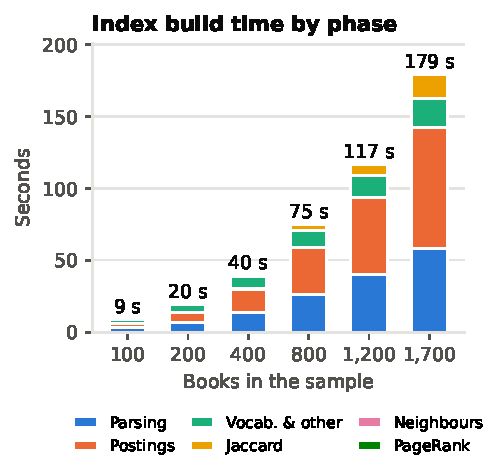
\includegraphics[width=\linewidth]{indexing_phases}
        \caption{Temps total par phase.}
        \label{fig:indexing-phases}
    \end{subfigure}\hfill
    \begin{subfigure}[t]{0.49\linewidth}
        \centering
        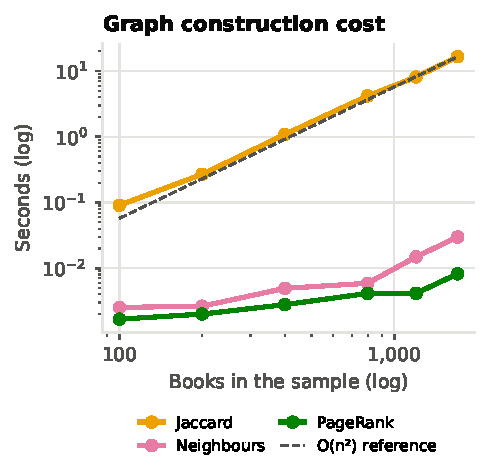
\includegraphics[width=\linewidth]{graph_scaling}
        \caption{Phases du graphe (échelles logarithmiques), avec une référence quadratique en pointillés.}
        \label{fig:graph-scaling}
    \end{subfigure}
    \caption{Temps de construction de l'index selon la taille de l'échantillon.}
    \label{fig:indexing}
\end{figure}

\paragraph{Temps de recherche.}
La figure~\ref{fig:query-latency} montre que la recherche par mot-clé est nettement plus rapide que la recherche par RegEx. Le temps d'une recherche par mot-clé dépend du nombre de livres qui contiennent le mot : plus ce nombre est grand, plus la recherche est lente, car il faut récupérer autant de lignes depuis la base de données, puis construire et trier les objets correspondants en Python. Pour les mots-clés, le classement par PageRank est généralement plus lent que le classement par occurrences : les occurrences sont déjà en mémoire depuis l'étape précédente, où elles ont été comptées, alors que le serveur ne conserve aucun état entre deux requêtes et doit donc relire dans la base les valeurs PageRank de tous les livres, ce qui prend environ 1~ms. Pour les RegEx, l'index en arbre B de la base de données ne peut pas accélérer une expression régulière : il faut donc charger tout le vocabulaire et tester chaque mot avec RE2 en Python, si bien que le temps dépend à peine de l'expression. Le chargement du vocabulaire représente environ un tiers de ce temps, et la correspondance mot par mot les deux tiers restants. Pour l'optimiser, on pourrait garder le vocabulaire en mémoire et réduire le nombre d'appels Python par mot.

Dans la figure~\ref{fig:query-scaling}, pour les mêmes raisons, la recherche par RegEx est nettement plus lente que la recherche par mot-clé quelle que soit la taille du corpus, et son temps augmente fortement avec le nombre de livres, mais moins vite que $n$. En effet, une RegEx parcourt tout le vocabulaire, et à mesure que des livres sont ajoutés, les mots encore absents du vocabulaire se font de plus en plus rares : le vocabulaire croît de plus en plus lentement, et le temps d'une RegEx aussi, puisqu'il est à peu près proportionnel à la taille du vocabulaire. La recherche par mot-clé, elle, s'effectue dans un arbre B dont la hauteur reste faible, et son temps reste stable, de l'ordre de quelques millisecondes.

\begin{figure}[H]
    \centering
    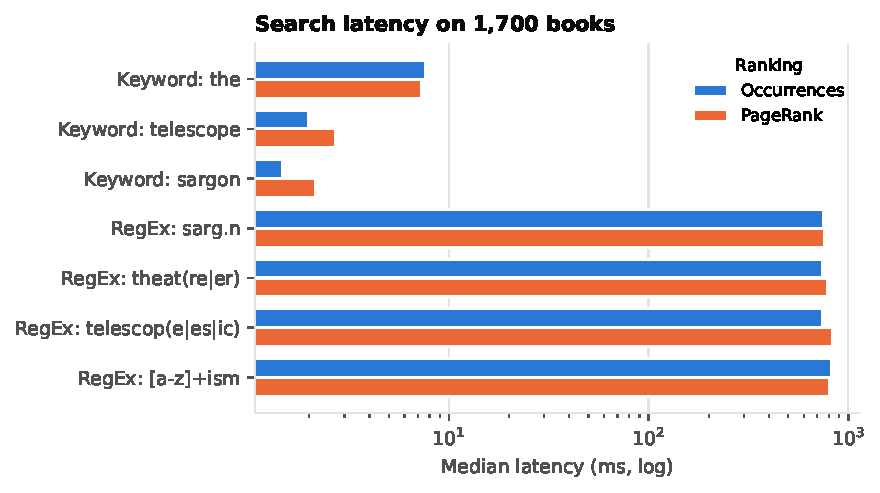
\includegraphics{query_latency}
    \caption{Latence médiane de chaque requête sur le corpus complet, pour les deux classements (échelle logarithmique).}
    \label{fig:query-latency}
\end{figure}

\begin{figure}[H]
    \centering
    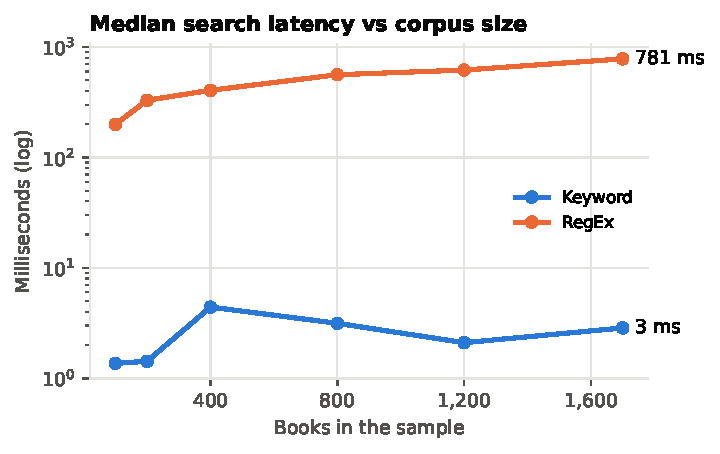
\includegraphics{query_scaling}
    \caption{Latence médiane des recherches selon la taille du corpus.}
    \label{fig:query-scaling}
\end{figure}

\paragraph{Test de charge.}
Nous avons enfin réalisé un test de charge : des threads Python simulent plusieurs utilisateurs qui lancent des recherches en même temps, en passant par Nginx. Le nombre de clients simultanés va de 1 à 32 ; pour les RegEx, il s'arrête à 8, car au-delà les requêtes dépassent le délai de 120~s de Nginx. Nous mesurons deux indicateurs : le débit et la latence. La figure~\ref{fig:stress} montre que le débit de la recherche par mot-clé atteint son maximum avec 2 clients, puis diminue, tandis que celui des RegEx diminue dès le départ. La cause la plus probable est la suivante : le serveur de développement de Django n'utilise qu'un seul processus, et le verrou global de l'interpréteur (GIL) de Python n'autorise qu'un seul thread à exécuter du code Python à la fois ; plus il y a de threads, plus les changements de contexte sont fréquents et coûteux. De plus, chaque requête RegEx charge tout le vocabulaire en mémoire : plus il y a de requêtes simultanées, plus la mémoire est sollicitée, ce qui accentue la baisse pour les RegEx.

La figure~\ref{fig:stress-latency} montre qu'avec 4 utilisateurs au plus, la recherche par mot-clé paraît instantanée (moins de 0,1~s, selon les seuils de Nielsen~\cite{nielsen}) ; avec 32 utilisateurs, sa latence médiane atteint environ 2~s, et l'attente devient nettement perceptible. La recherche par RegEx, elle, demande environ 0,8~s même avec un seul utilisateur, et dépasse 10~s dès 4 utilisateurs, ce qui la rend pratiquement inutilisable.

\begin{figure}[H]
    \centering
    \begin{subfigure}[t]{0.49\linewidth}
        \centering
        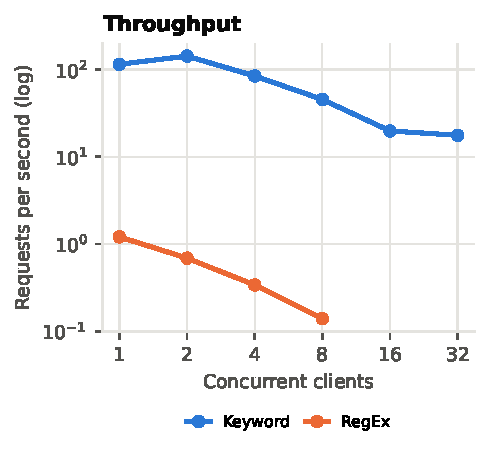
\includegraphics[width=\linewidth]{stress_throughput}
        \caption{Débit (requêtes traitées par seconde).}
        \label{fig:stress-throughput}
    \end{subfigure}\hfill
    \begin{subfigure}[t]{0.49\linewidth}
        \centering
        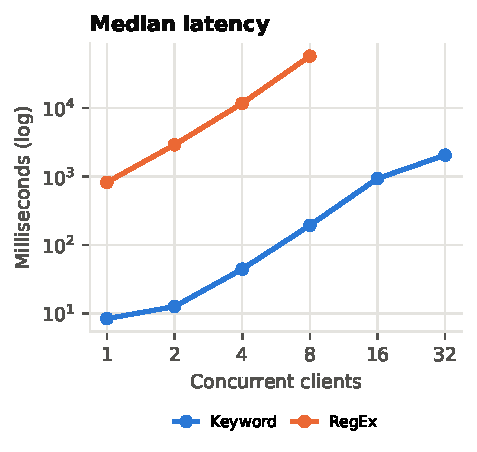
\includegraphics[width=\linewidth]{stress_latency}
        \caption{Latence médiane d'une requête.}
        \label{fig:stress-latency}
    \end{subfigure}
    \caption{Débit et latence de l'API selon le nombre de clients simultanés, requêtes envoyées à travers Nginx (échelles logarithmiques). Au-delà de 8 clients, les RegEx dépassent le délai de 120~s de Nginx.}
    \label{fig:stress}
\end{figure}

% Figures facultatives, si la place le permet :
% 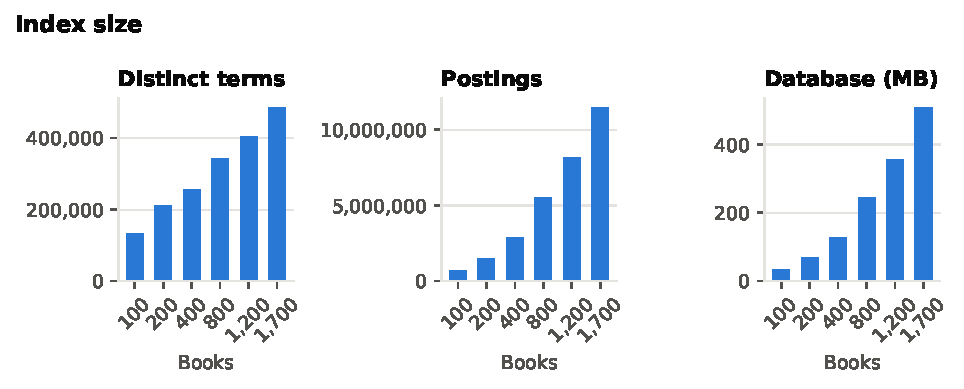
\includegraphics{index_growth}       % taille de l'index
% 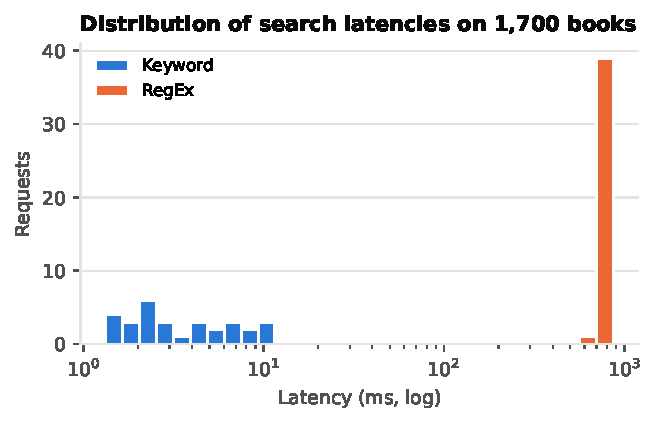
\includegraphics{latency_histogram}  % distribution des latences

\subsection{Tests de pertinence}

\paragraph{Objectif.}
Nous évaluons ensuite la pertinence des résultats obtenus, afin de savoir si les livres placés en tête des résultats correspondent bien à l'intention de l'utilisateur. La pertinence d'un livre est jugée de deux façons : d'une part à la main par les membres de l'équipe, un livre étant jugé pertinent dès qu'un membre le considère comme tel ; d'autre part à partir des étiquettes (catégories) du catalogue Gutenberg.

\paragraph{Méthode.}
Nous avons effectué cinq recherches par mot-clé, chacune représentant un besoin différent. \texttt{holmes} désigne un personnage célèbre et une série ; cette requête devrait être facile, car le mot \texttt{holmes} devrait apparaître très souvent dans les livres de la série, qui sont aussi les plus pertinents. \texttt{detective} permet de vérifier si les livres trouvés sont des romans policiers. \texttt{love} cherche des romans d'amour : ce mot apparaît dans presque tous les livres, si bien que son nombre d'occurrences distingue mal ces romans, mais les étiquettes aident à les reconnaître. \texttt{chemistry} cherche des livres de chimie, et \texttt{sargon} un personnage historique. Pour chaque requête et chaque classement, nous examinons les 5 premiers résultats, soit 50 résultats, ainsi que les 3 premières recommandations, soit 30 recommandations. Selon les étiquettes, un livre est pertinent si l'une de ses étiquettes Subjects ou Bookshelves contient le mot recherché ; comme \texttt{sargon} n'apparaît dans aucune étiquette, un livre est alors pertinent si ses étiquettes mentionnent Babylone ou l'Assyrie.

\paragraph{Résultats.}
Les résultats sont présentés dans la figure~\ref{fig:relevance-results} pour les résultats de recherche et dans la figure~\ref{fig:relevance-recommendations} pour les recommandations.

\begin{figure}[H]
    \centering
    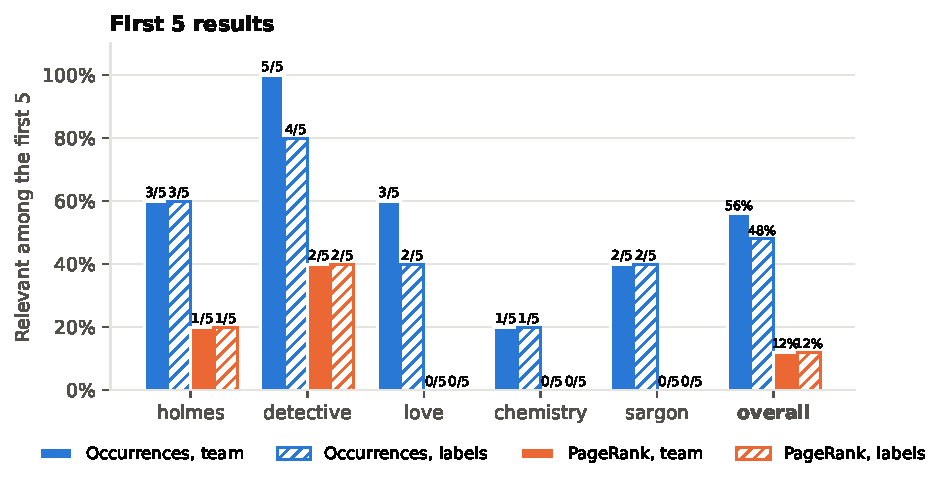
\includegraphics{manual}
    \caption{Proportion de livres pertinents parmi les 5 premiers résultats, pour les deux classements. Barres pleines : jugement de l'équipe ; barres hachurées : étiquettes du catalogue Gutenberg (un livre est pertinent si l'une de ses étiquettes contient le mot recherché ; pour \texttt{sargon}, si elle mentionne Babylone ou l'Assyrie).}
    \label{fig:relevance-results}
\end{figure}

\begin{figure}[H]
    \centering
    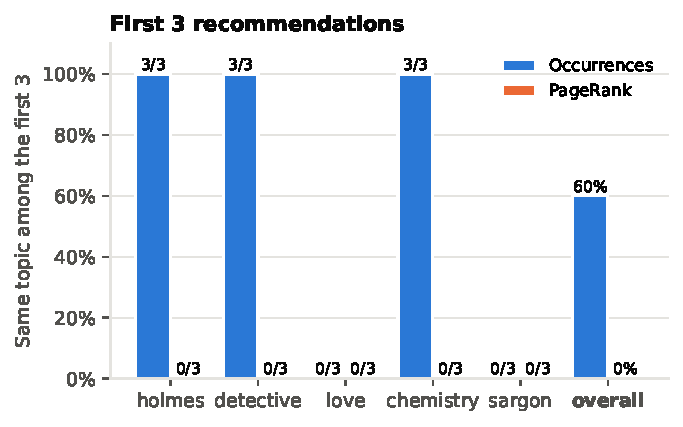
\includegraphics{recommendations}
    \caption{Proportion des 3 premières recommandations jugées du même thème que la requête par l'équipe, selon le classement qui fournit les livres de départ.}
    \label{fig:relevance-recommendations}
\end{figure}

\paragraph{Analyse.}
Le classement par occurrences est nettement meilleur que le classement par PageRank, car PageRank mesure l'importance d'un livre dans toute la bibliothèque, indépendamment de la requête. Le principal défaut du classement par occurrences est de ne pas tenir compte de la longueur des livres : plus un livre est long, plus le mot recherché y apparaît souvent (par exemple, le premier résultat de \texttt{love} est l'œuvre complète de Shakespeare). Enfin, les étiquettes se révèlent assez fiables, puisqu'elles concordent avec le jugement de l'équipe dans 96~\% des cas ; on pourrait à l'avenir en tenir compte dans le classement, par exemple en augmentant le score des livres dont les étiquettes contiennent le mot recherché.

Pour les recommandations (figure~\ref{fig:relevance-recommendations}), le mot \texttt{love} apparaît dans presque tous les livres : les premiers résultats sont déjà peu pertinents, et les recommandations le sont donc aussi. Mais le phénomène le plus net est que les recommandations échouent complètement lorsqu'elles partent du classement par PageRank : elles sont formées des voisins, dans le graphe de Jaccard, des premiers livres classés, et comme ces premiers livres ne sont déjà pas pertinents avec PageRank, les recommandations ne peuvent pas l'être non plus.

% ---------------------------------------------------------------- ~1 page
\section{Discussion et limites}

% ---------------------------------------------------------------- ~0,5 page
\section{Conclusion et perspectives}
% Conclusion : à rédiger.

\paragraph{Perspectives.}
\begin{enumerate}
    \item Remplacer le serveur de développement de Django par un serveur multiprocessus comme Gunicorn : chaque processus possède son propre GIL, si bien que plusieurs requêtes peuvent réellement être traitées en parallèle.
    \item Garder le vocabulaire en mémoire, pour ne pas le recharger à chaque recherche par RegEx.
    \item Le classement par occurrences favorise les livres longs. On pourrait le remplacer par un score TF-IDF : diviser le nombre d'occurrences par la longueur du livre (TF) supprime cet avantage, et pondérer chaque mot par $\log(N/\mathrm{df})$, où $\mathrm{df}$ est le nombre de livres qui le contiennent (IDF), réduit le poids des mots trop courants lorsqu'une RegEx en trouve plusieurs.
    \item PageRank donne de mauvais résultats dans notre projet : sur le graphe de Jaccard, il désigne surtout les livres dont le vocabulaire est le plus typique, c'est-à-dire les plus semblables aux autres, indépendamment de la requête. On pourrait le rendre dépendant de la requête (PageRank personnalisé~\cite{pagerank}) : lors d'un saut aléatoire, le surfeur ne va que vers les livres trouvés, en proportion de leur score TF-IDF, ce qui mesure la centralité d'un livre parmi les livres de la requête. On pourrait aussi construire un graphe à partir des clics des utilisateurs (par exemple en reliant les livres cliqués lors d'une même recherche) et y calculer PageRank. Le score refléterait alors les livres que les utilisateurs jugent réellement utiles, ce qui est plus proche du sens original de PageRank sur le Web, où un lien vaut une recommandation.
\end{enumerate}

\begin{thebibliography}{9}
    \bibitem{pagerank} L.~Page, S.~Brin, R.~Motwani et T.~Winograd. \emph{The PageRank Citation Ranking: Bringing Order to the Web}. Rapport technique, Stanford InfoLab, 1999.
    \bibitem{jaccard} P.~Jaccard. Étude comparative de la distribution florale dans une portion des Alpes et du Jura. \emph{Bulletin de la Société Vaudoise des Sciences Naturelles}, 37, p.~547--579, 1901.
    \bibitem{re2} R.~Cox. \emph{Regular Expression Matching Can Be Simple And Fast}. 2007. \url{https://swtch.com/~rsc/regexp/regexp1.html}
    \bibitem{iir} C.~D.~Manning, P.~Raghavan et H.~Schütze. \emph{Introduction to Information Retrieval}. Cambridge University Press, 2008.
    \bibitem{nielsen} J.~Nielsen. \emph{Usability Engineering}. Academic Press, 1993.
    \bibitem{joel} J.~Spolsky. \emph{The Joel Test: 12 Steps to Better Code}. 2000. \url{https://www.joelonsoftware.com/2000/08/09/the-joel-test-12-steps-to-better-code/}
\end{thebibliography}

\end{document}
